\chapter{Hardware und Software}
Dieses Kapitel führt die gegebenen und verwendeten Hard- und Software Komponenten in dieser Arbeit auf.

\section{Der Kaffeevollautomat}

\subsection{Aufbau und Verkabelung}
\begin{figure}
  \begin{center}
    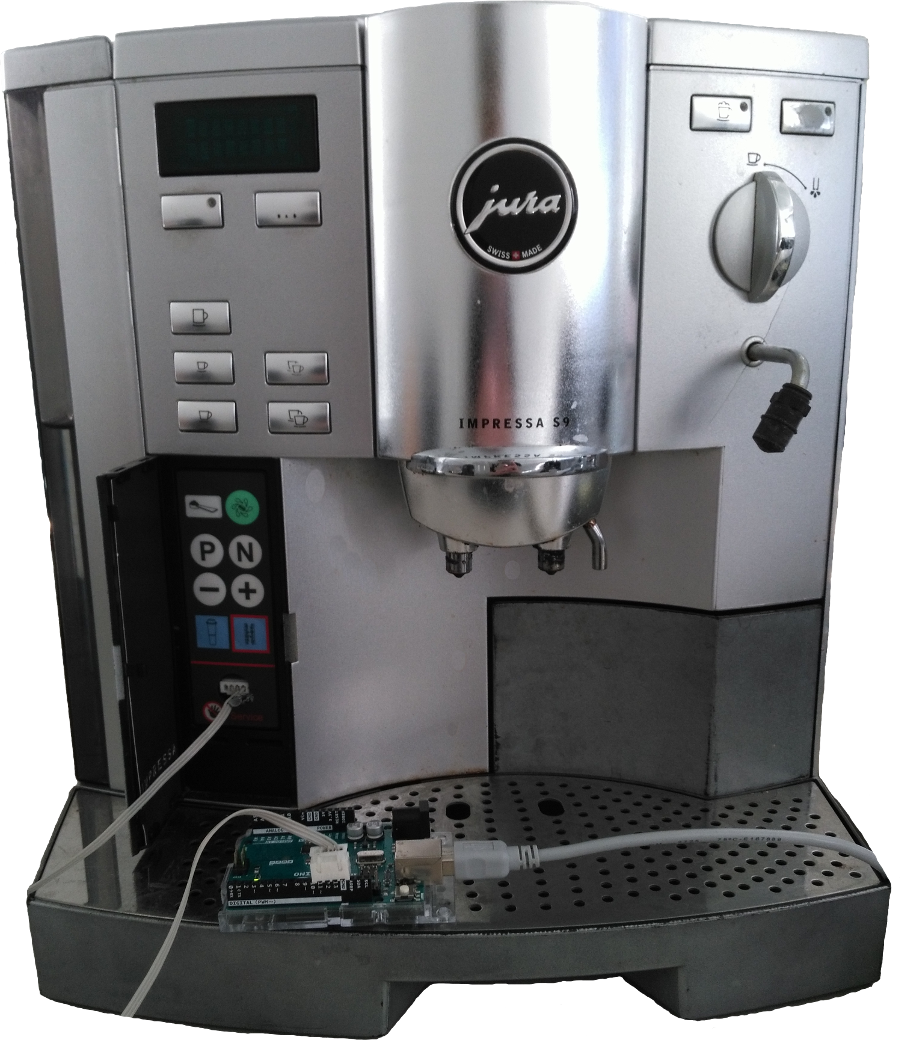
\includegraphics[scale=0.2]{images/Jura-Impressa-S9-small}
    \caption{Jura Impressa S9 -- Kaffeevollautomat}
    \label{fig:Kaffeevollautomat}
  \end{center}
\end{figure}

\begin{figure}
  \begin{center}
    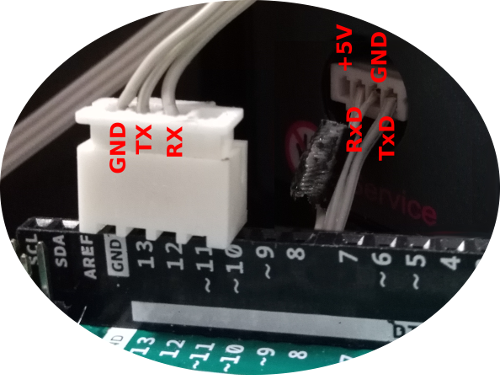
\includegraphics[scale=0.3]{images/Jura-Arduino-Pins-beschriftet-small}
    \caption{Pinbelegung: Jura Impressa S9 -- Arduino Uno}
    \label{fig:KaffeevollautomatPins}
  \end{center}
\end{figure}

Der "`Jura Impressa S9"', siehe Abbildung \ref{fig:Kaffeevollautomat}, ist ein Kaffeevollautomat mit fünf Kaffeebezugstasten (Spezialkaffee, 1 große Tasse Kaffee, 2 große Tassen Kaffee, 1 kleine Tasse Kaffee und 2 kleinen Tassen Kaffee).
Auf der rechten Seite befinden sich Tasten für heißes (Tee-)Wasser und Wasserdampf zum Milch Aufschäumen.
Interessanter wird es hinter der linken Wartungsklappe. Dort befindet sich neben mehreren Menü-Tasten auch eine serielle Schnittstelle.
Über ein eigenes \ac{UART} Protokoll, siehe Kapitel \ref{subsec:SerielleKommunikation}, kann hierüber mit der Maschine kommuniziert werden.
Ein Arduino Uno übersetzt als "`Man in the middle"' die bekannten Kommandos in das Format der Kaffeemaschine. Über eine weitere serielle Verbindung über USB lässt sich der Arduino ansteuern. Aus Sicht des Computers ist der Arduino ein Gerätelaufwerk unter \texttt{/dev/ttyACM0} mit einer Baudrate von 9600. Diese Zahl findet sich zu Beginn des Arduino Skrips wieder. \todo verweis aufs Ardunio Skript, Projekt CoffeeMachine.

\subsection{Kommandos}
Die Tabelle~\ref{tbl:kommandos} zeigt die Befehlsgruppen, sowie ausgewählte Befehle, die der Kaffeevollautomat versteht.

\begin{tuhhtable}
  \footnotesize\centering
  \begin{tabular}[tp]{L{.22\textwidth}L{.48\textwidth}L{.18\textwidth}}
%
  \THc{1}{c}{Kommando} & \THc{1}{c}{Beschreibung} & \THc{1}{c}{Rückgabewert} \\
%
  \TRx{3}{l}{Betriebszustand (AN:<id>)}\\
  \abovebodyrule
  AN:01    & Einschalten        & ok:    \\\TRc
  AN:02    & Ausschalten        & ok:    \\
  AN:03    & Display Test       & ok:    \\\TRc
  AN:<id>  & u.v.m.             & ok:    \\
  \belowbodyrule
%
  \TRx{3}{l}{Bezugstaste (FA:<id>)}\\
  \abovebodyrule
  FA:02    & Gerät spülen       & ok:    \\\TRc
  FA:0C    & Spezialkaffee      & ok:    \\
  FA:<id>  & u.v.m.             & ok:    \\\TRc
  \belowbodyrule
%
  \TRx{3}{l}{Steuerungskomponenten (FN:<id>)}\\
  \abovebodyrule
  FN:<id>  & Pumpen, Heizung, u.v.m & ok:    \\\TRc
  \belowbodyrule
%
  \TRx{3}{l}{Eingabestatus*}\\
  \abovebodyrule
  IC:      & Eingaben auslesen* &        \\\TRc
  \belowbodyrule
%
  \TRx{3}{l}{Spiele Musik (easter egg)*}\\
  \abovebodyrule
  PM:      & Play music*        &        \\\TRc
  \belowbodyrule
%
  \TRx{3}{l}{Speicherzugriff}\\
  \abovebodyrule
  RE:<address> & Liest 2 Byte EEPROM Speicher   & re:[0000-FFFF] \\\TRc
  WE:<address>,<value> & Schreibt 2 Byte in EEPROM & ok:         \\
  RT:<address> & Liest eine Zeile EEPROM        & rt:[0-F 64x]   \\\TRc
  RR:<address> & Liest eine Zeile RAM           & rr:[0-F 32x]   \\
  \belowbodyrule
%
  \TRx{3}{l}{Sperrung}\\
  \abovebodyrule
  ?M3      & Aktiviert den Inkassomodus         & ?ok            \\\TRc
  ?M1      & Deaktiviert den Inkassomodus       & ?ok            \\
  \belowbodyrule
%
  \TRx{3}{l}{Display}\\
  \abovebodyrule
  ?D0      & Standard Displaytext zurück setzen & ?ok            \\\TRc
  ?D1[A-Z 8-11x] & Displaytext Zeile 1          & ?ok            \\
  ?D2[A-Z 8-11x] & Displaytext Zeile 2          & ?ok            \\\TRc
  \belowbodyrule
%
  \TRx{3}{l}{Aktion an der Kaffeemaschine}\\
  \abovebodyrule
           & 1 kleiner Kaffee (Produkt 1)       & ?PAE         \\\TRc
           & 2 kleine Kaffees (Produkt 2)       & ?PAF         \\
           & 1 großer Kaffee  (Produkt 3)       & ?PAA         \\\TRc
           & 2 große Kaffees  (Produkt 4)       & ?PAB         \\
           & Spezialkaffe     (Produkt 7)       & ?PAG         \\\TRc
           & Dampf            (Produkt 6)       & ?PAI         \\
           & 1 Dampfportion   (Produkt 5)       & ?PAJ         \\\TRc
           & 1 Tasse Tee      (Produkt 8)       & ?PAK         \\
  \belowbodyrule
%
  \TRx{3}{l}{* leider nicht alles in der Jura Impressa S9 implementiert, siehe weitere Geräte der S-Reihe}\\
%
  \end{tabular}
  \caption{Befehlsübersicht der Jura Kaffeevollautomaten (S-Reihe)}
  \label{tbl:kommandos}
\end{tuhhtable}


\section{Bibliotheken}

\subsection{Serielle Kommunikation}\label{subsec:SerielleKommunikation}
Aus dem Projekt "`CoffeeMachine"'\footnote{\label{GitlabProject_CoffeeMachine}\href{https://collaborating.tuhh.de/e-17/General/CoffeeMachine}{https://collaborating.tuhh.de/e-17/General/CoffeeMachine}} stammt das Programm des Arduino UNO zum Kodieren der \ac{UART} Kommandos. Die an den Kaffeevollautomaten adressierten Bytes (ASCII-Zeichen für Zeichen der Befehle aus der Kommando Tabelle~\ref{tbl:kommandos}), bestehend aus seinen acht Bits, werden in je vier Bytes aufgeteilt. Die dritte und sechste Stelle der neuen Bytes repräsentieren je zwei Bits des ursprünglichen Bytes. Bei der Übertragung an den Kaffeevollautomaten werden die restlichen Bits mit Nullen aufgefüllt. Abbildung \ref{fig:uart} veranschaulicht dies an dem ersten Byte des Einschaltbefehls.
Die Kodierung der, von dem Kaffeevollautomaten kommenden, Bytes erfolgt analog. Laut "`Protocoljura"'\footnote{\url{http://protocoljura.wiki-site.com/index.php/Protocol_to_coffeemaker}} bestehen die irrelevanten Bits der ankommenden Bytes aus einer Null und weiteren fünf Einsen pro Byte.

Vier Bytes kodieren ein ASCII Zeichen und werden fortan als Gruppe bezeichnet. Zwischen jeder Gruppe gibt es eine Verzögerung von 8ms. Diese Verzögerung begrenzt hauptsächlich die Übertragungsgeschwindigkeit, was in Abschnitt \ref{subsec:zugangSeriellDirekt} diskutiert wird.

Die jetzt vorhandene Umgebung kann bereits über den seriellen Monitor der Arduino IDE genutzt werden.

\begin{figure}
  \begin{center}
    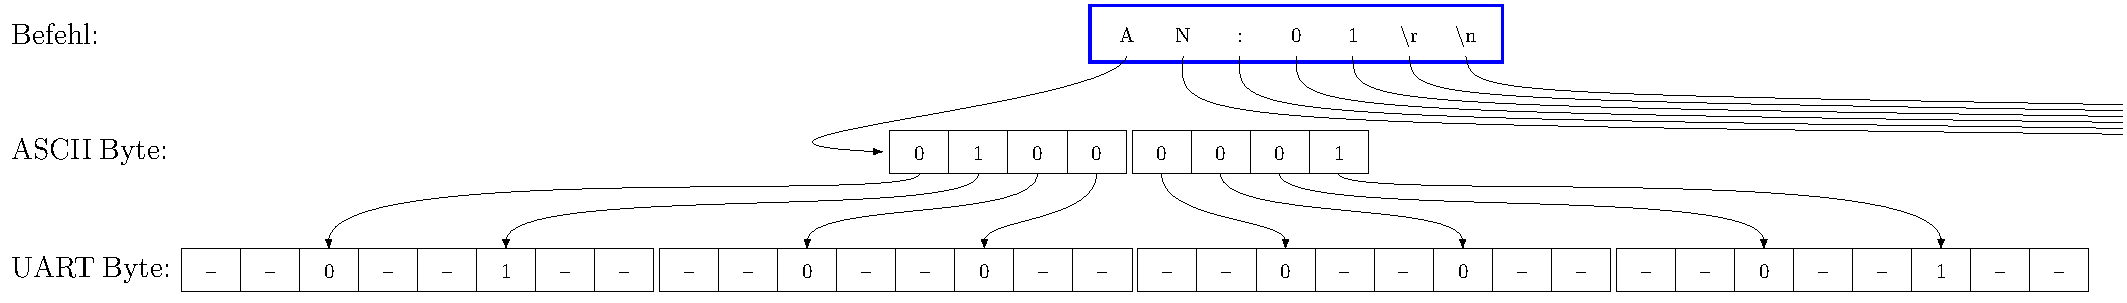
\includegraphics[scale=0.4]{images/UART-Bytes}
    \caption{Umrechnung }
    \label{fig:uart}
  \end{center}
\end{figure}

\subsubsection{libserial}

\subsection{Speicherformat}

\subsubsection{libjsoncpp}



